\documentclass[11pt]{article}

% Mode is controlled by the `acl-mode` YAML field:
%   review   — anonymous, line numbers (default for submission)
%   final    — camera-ready, authors shown
%   preprint — non-anonymous, page numbers
% acl.sty handles: geometry (a4, 2.5cm margins), twocolumn, natbib,
%   caption, hyperref, bibliographystyle{acl_natbib}.
% Do NOT load those packages again here.
% Pass sort option to natbib before acl.sty loads it
\PassOptionsToPackage{sort}{natbib}
\usepackage[review]{acl}

% Packages from the official ACL template (acl_latex.tex) — safe to load after acl.sty
\usepackage{times}
\usepackage{latexsym}
\usepackage[T1]{fontenc}
\usepackage[utf8]{inputenc}
\usepackage{textcomp}   % euro sign and other symbols
\usepackage{microtype}
\usepackage{inconsolata}

% Math
\usepackage{amsmath}
\usepackage{amssymb}

% Tables — all three needed for pandoc's longtable output
\usepackage{longtable}
\usepackage{booktabs}
\usepackage{array}     % pandoc uses >{\raggedright\arraybackslash}p{} column types
\usepackage{calc}      % pandoc uses \real{} expressions for column widths
\usepackage{multirow}  % multi-row table cells

% longtable is incompatible with twocolumn mode (enforced by acl.sty).
% Use etoolbox hooks to temporarily switch to onecolumn around each longtable.
% The table will appear full-width on its own page segment.
\usepackage{etoolbox}
\BeforeBeginEnvironment{longtable}{\onecolumn}
\AfterEndEnvironment{longtable}{\twocolumn}

% Fix table caption numbering for longtable
\def\fnum@table{\tablename~\thetable}

% Graphics
\usepackage{graphicx}
\makeatletter
% pandoc uses \maxwidth and \maxheight when including images
\def\maxwidth{\ifdim\Gin@nat@width>\linewidth\linewidth\else\Gin@nat@width\fi}
\def\maxheight{\ifdim\Gin@nat@height>\textheight\textheight\else\Gin@nat@height\fi}
% Default figure placement
\def\fps@figure{htbp}
\makeatother

% Code blocks and inline code
\IfFileExists{upquote.sty}{\usepackage{upquote}}{}  % straight quotes in verbatim
\usepackage{fancyvrb}
\newcommand{\passthrough}[1]{#1}  % pandoc inline code

% Suppress date (ACL papers do not display a date)
\date{}

% pandoc: scale images to fit column width, preserving aspect ratio
\makeatletter
\newsavebox\pandoc@box
\newcommand*\pandocbounded[1]{%
  \sbox\pandoc@box{#1}%
  \Gscale@div\@tempa{\linewidth}{\wd\pandoc@box}%
  \ifdim\@tempa\p@<\p@\scalebox{\@tempa}{\usebox\pandoc@box}\else#1\fi%
}
\makeatother

% pandoc: tight lists (no extra space between items)
\providecommand{\tightlist}{%
  \setlength{\itemsep}{0pt}\setlength{\parskip}{0pt}}

\title{Instructions for ACL Proceedings}

% In review mode, acl.sty replaces the author block with
% "Anonymous ACL submission" automatically.
\author{
  Alice Smith \\
      University of Nowhere \\
        \texttt{alice.smith@nowhere.edu}
     \And
  Bob Jones \\
      Institute of Made-Up Science \\
        \texttt{bob.jones@madeup.edu}
    }

\begin{document}
\maketitle

\begin{abstract}
This document contains instructions for preparing a submission to ACL
and affiliated venues using the \textbf{acl} Quarto template. It also
serves as a demonstration of the template's formatting: the document you
are reading is itself typeset using the template. Replace the YAML
fields above and the section content below with your own manuscript.
\end{abstract}

\section{Installation}\label{installation}

The easiest way to install this template is directly from GitHub. Run
the following command from your project directory:

\begin{verbatim}
quarto add znhoughton/quarto-templates/acl
\end{verbatim}

Alternatively, if you have a local clone of the repository, you can
install from the local path instead:

\begin{verbatim}
quarto add "path/to/quarto-templates/acl"
\end{verbatim}

Either method copies the \texttt{\_extensions/acl/} folder into your
project. Once installed, set the format in your document's YAML front
matter:

\begin{verbatim}
format:
  acl-pdf: default
\end{verbatim}

Then render with:

\begin{verbatim}
quarto render your-document.qmd
\end{verbatim}

The extension folder is self-contained and can be committed to your
repository so that collaborators do not need a separate installation
step. The \texttt{\_extensions/} folder should not be listed in
\texttt{.gitignore} if you want the template to be available to everyone
who clones the repository. To update the template to the latest version
at any time, simply re-run the \texttt{quarto\ add} command from above.

\section{Text Formatting}\label{text-formatting}

This document is typeset using the \texttt{acl} template. The body text
you are reading demonstrates the default two-column layout, font, and
spacing. Inline formatting options include \textbf{bold}, \emph{italic},
\texttt{inline\ code}, and \textsc{small caps}.

Long tables and figures can span both columns using the \texttt{table*}
and \texttt{figure*} LaTeX environments in a raw LaTeX block. Paragraphs
are separated by a blank line. A single line break within a paragraph
does not produce a new paragraph.

The ACL template uses Times Roman for the body text and Helvetica for
line numbers. Font size is 11pt with two-column layout. Line spacing and
margins are set by \texttt{acl.sty} and should not be overridden. Do not
add custom geometry, font, or spacing commands to your document.

Section headings use \texttt{\#} for top-level sections and
\texttt{\#\#} for subsections. ACL papers do not typically use headings
deeper than \texttt{\#\#\#}. The template numbers sections
automatically; do not add manual numbering to heading text
\citep{Smith2020}.

\section{Tables}\label{tables}

Use an R chunk with \texttt{knitr::kable()} and the
\texttt{\#\textbar{}\ label:} and \texttt{\#\textbar{}\ tbl-cap:} chunk
options to produce tables.

\begin{table}

\centering{

\begin{tabular}{lrr}
\toprule
Condition & Mean & SD\\
\midrule
A & 1.2 & 0.3\\
B & 2.4 & 0.5\\
\bottomrule
\end{tabular}

}

\caption{\label{tbl-example}A simple table showing condition means.}

\end{table}%

Cross-reference with \texttt{@tbl-example}, which produces
Table~\ref{tbl-example}. Tables that span both columns use a
\texttt{table*} environment in a raw LaTeX block. Keep single-column
tables narrow enough to fit within one column width; use the
\texttt{table*} environment only when the content genuinely requires the
full page width.

\section{Figures}\label{figures}

Use an R chunk with \texttt{\#\textbar{}\ label:\ fig-xxx} and
\texttt{\#\textbar{}\ fig-cap:} chunk options to produce figures with
captions and cross-reference labels.

\begin{figure}

\centering{

\pandocbounded{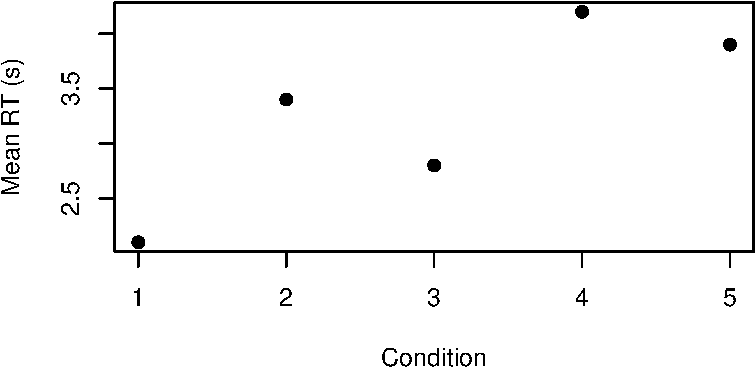
\includegraphics[keepaspectratio]{example_acl_files/figure-pdf/fig-example-1.pdf}}

}

\caption{\label{fig-example}A simple scatter plot for illustration.}

\end{figure}%

Cross-reference with \texttt{@fig-example}, which produces
Figure~\ref{fig-example}. Wide figures can span both columns using a
\texttt{figure*} environment in a raw LaTeX block. Figures are floating
by default and will be placed at the top or bottom of the nearest page.
For publication-quality plots, prefer vector formats (PDF or SVG) over
raster formats (PNG, JPEG) to ensure sharpness at any print resolution.

\section{Equations}\label{equations}

Inline math: \(y = \beta_0 + \beta_1 x + \varepsilon\).

Display equation:

\begin{equation}\phantomsection\label{eq-model}{
Y_{ij} = \beta_0 + \beta_1 X_{ij} + u_i + \varepsilon_{ij}
}\end{equation}

Cross-reference with \texttt{@eq-model}, which produces
Equation~\ref{eq-model}.

Multi-line display equations:

\[
\mu_i = \alpha + \beta x_i, \quad y_i \sim \mathcal{N}(\mu_i, \sigma^2)
\]

Use display equations for any expression that is important enough to be
referred to by number. Number only equations that are actually
cross-referenced in the text; unnumbered display equations use the plain
\texttt{\$\$...\$\$} syntax without a label.

The \texttt{amsmath} package is loaded by the template and provides
environments such as \texttt{align}, \texttt{gather}, and \texttt{cases}
via raw LaTeX blocks. Inline math uses standard \texttt{\$...\$}
delimiters. Avoid mixing LaTeX math commands with Pandoc markdown
constructs in the same expression.

\section{Submission Modes}\label{submission-modes}

Change \texttt{acl-mode} in the YAML front matter to switch modes:

\begin{table}

\centering{

\begin{tabular}{llll}
\toprule
Mode & Authors & Lines & Use\\
\midrule
review & anonymous & yes & submission\\
final & shown & no & camera-ready\\
preprint & shown & no & arXiv\\
\bottomrule
\end{tabular}

}

\caption{\label{tbl-modes}ACL submission modes.}

\end{table}%

In \texttt{review} mode the document is anonymised and line numbers are
added for reviewer reference. The author list is replaced with
``Anonymous ACL submission.'' In \texttt{final} mode, authors and
affiliations are shown and line numbers are removed. Use
\texttt{preprint} for posting to arXiv or a personal website before the
camera-ready deadline. Switch modes by changing a single YAML field; no
other changes to the document are needed.

Remember to remove or anonymise any self-identifying references in the
manuscript body before submitting in \texttt{review} mode. This includes
references to your own prior work that would reveal authorship, links to
personal repositories, and acknowledgements. Restore these for the
\texttt{final} camera-ready version.

% acl.sty sets \bibliographystyle{acl_natbib} at load time.
% Only \bibliography{} is needed here to point to the bib file(s).
\bibliography{example.bib}

\end{document}
